% \vspace{-0.6\baselineskip}
\section{Introduction}
% \vspace{-0.4\baselineskip}
\label{sec:intro}

With the advances of deep learning techniques and increase in dataset collections, there have been successes in scaling up object classification systems. However, unlike object class labeling, tedious bounding boxes annotation, which is required for supervised object detection, is hardly scalable. 
% Besides, videos provide richer information than static images and can be leveraged for learning. 
Recently, there have been impressive progresses in unsupervised and weakly supervised object detection, making the pipeline free of bounding box supervision. However, existing unsupervised methods show much inferior performance compared to supervised methods. And the weakly supervised ones, which are mostly trained on static images, often fail to generalize to videos due to domain shift. In light of this, we investigate the problem of ``weakly supervised object detection by learning from videos with action labels''. Instead of using boudning box annotations in fully-supervised pipeline or video-level object class in previous weakly supervised method, we use video-level action class annotation for supervision, as it is easy to obtain and commonly appears in existing video datasets. During training, only videos with action labels are used. For evaluation, static images are fed into the pipeline and spatial bounding boxes with object classes will be estimated.

% \begin{figure}
% % \vspace{-0.5\baselineskip}
% 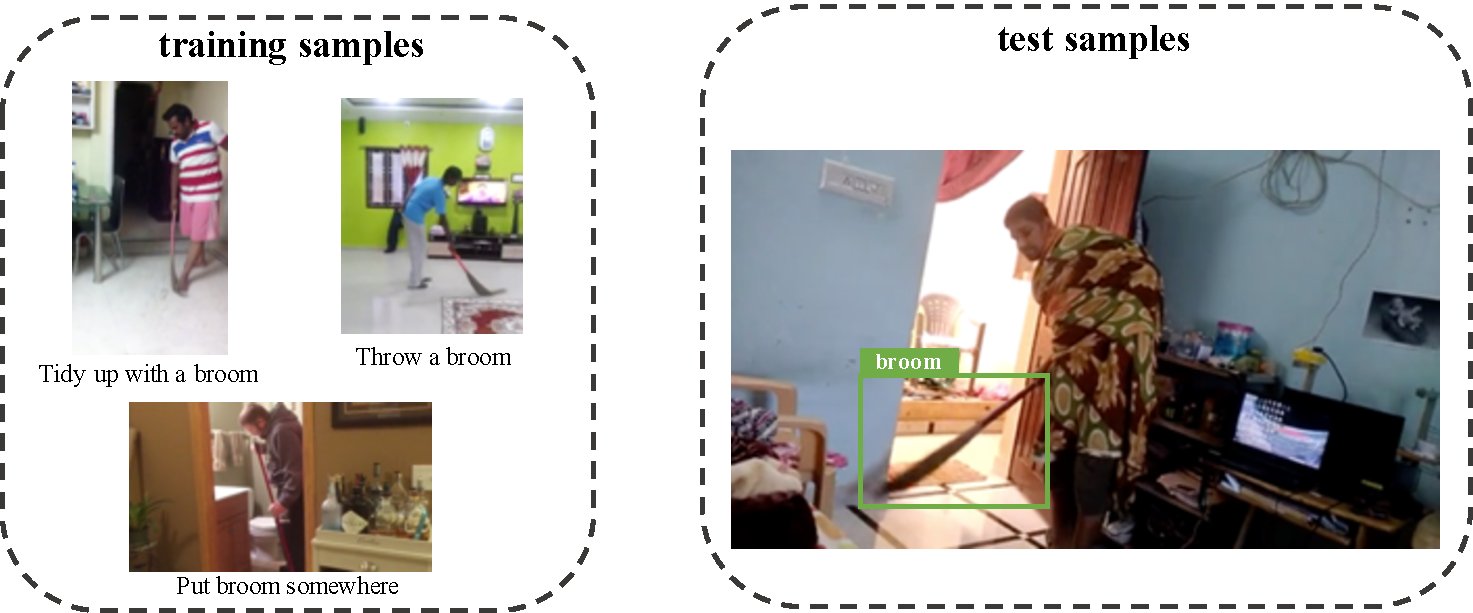
\includegraphics[width=0.5\textwidth]{figures/training_test_samples.pdf}
% % \caption{Visual comparison of depth and normal results between \protect\cite{zhou2017unsupervised} and ours. As the original depth ground truth map comes from sparse laser measurement, the interpolated depth map is shown for better visualization. As can be seen from the depth estimation, our results preserve the small/thin structures which have similar color to other foregrounds (green circles). From the normal comparison, our results predict the road normal direction better and have no artifact. The edges in normal map are also preserved better in our results (yello circles).}
% \caption{Train samples include videos with action labels. Bounding boxes and object class are estimated during evaluation.}
% % \vspace{-0.8\baselineskip}
% \label{fig:train_samples}
% \end{figure}

\begin{figure*}
% \vspace{-0.5\baselineskip}
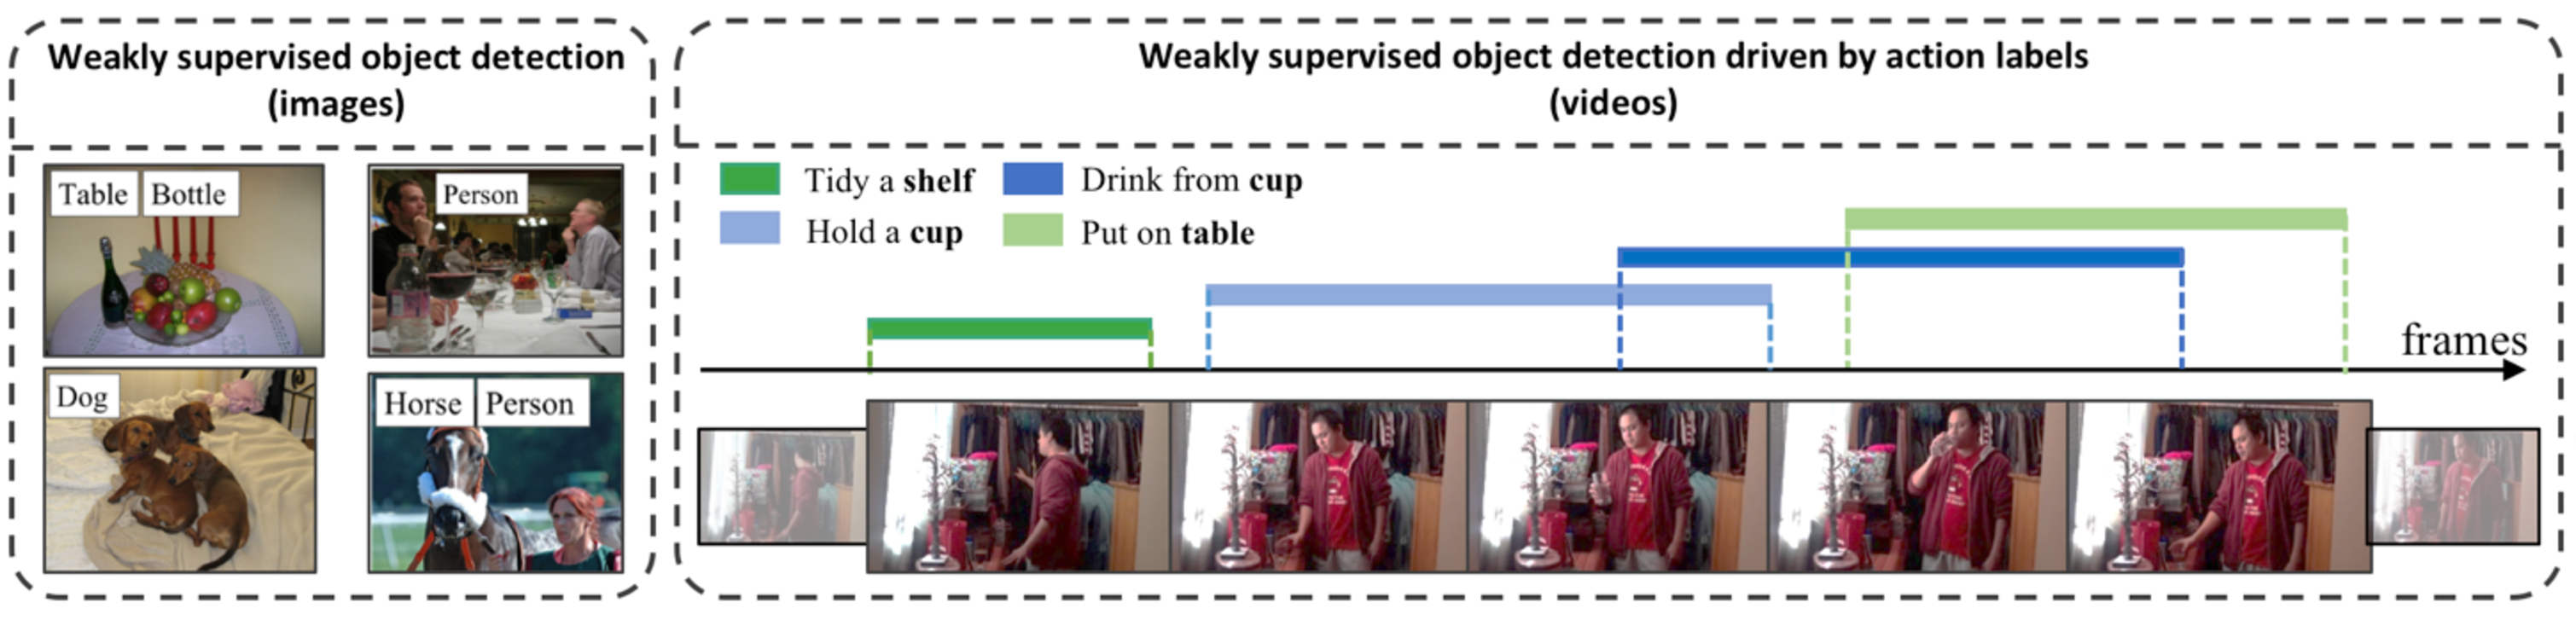
\includegraphics[width=1.0\textwidth]{figures/task_definition.pdf}
% \caption{Visual comparison of depth and normal results between \protect\cite{zhou2017unsupervised} and ours. As the original depth ground truth map comes from sparse laser measurement, the interpolated depth map is shown for better visualization. As can be seen from the depth estimation, our results preserve the small/thin structures which have similar color to other foregrounds (green circles). From the normal comparison, our results predict the road normal direction better and have no artifact. The edges in normal map are also preserved better in our results (yello circles).}
\caption{Traditional weakly supervised object detection takes images with image-level object classes as training samples. Our task takes video with clip-level action labels as ground truth for training.}
% \vspace{-0.8\baselineskip}
\label{fig:task_definition}
\end{figure*}

Previous work \cite{yuan2017temporal} proposed to cope with the problem by leveraging temporal consistency of object proposals and use the object class that appears in the action name (\eg ``cup'' in the action ``drink from cup'') as video-level object labels for supervising the learning of object appearance. Specifically, the class-agnostic object proposals are generated using EdgeBoxes \cite{zitnick2014edge}. The proposals are linked in temporal space by measuring the appearance feature similarity. The appearance feature is updated recurrently by incorporating the information from neighboring frames using LSTM. The updated features are then fed into a two-stream classification module as in \cite{bilen2016weakly} and the related object class in action label is used for classification supervision. Such method only parses the object class from action class labels and fails to model the human action motion or the interaction between human and objects.

In this work, we are solving the drawbacks mentioned above. Our ideas are mainly motivated by three observations: (1) The object appearance is consistent across videos and across action classes which involve the same object class; (2) There is spatial correlation between the motions of objects and human key points, \eg in action ``hold cup'', the location of cup is tightly correlated with location of the hand. And such correlation is dependent on action class; (3) The most informative object in the scene of a certain action class is the interacted object and thus the action class can be leveraged for object appearance modeling. The most dominant challenge in this task is the large space and few supervision signal. We try to formulate our proposed method to decrease the search space based on the above observations: (1) use generic object classifier for modeling object appearances, (2) learn an attention ditribution to model the probability of object locations \wrt the human joint, (3) jointly learn action and object classification to leverage the action cues.

We conducted comprehensive experiments over the Charades dataset \cite{sigurdsson2016hollywood} and show that our method outperforms the previous methods \cite{bilen2016weakly,yuan2017temporal} by a large margin on both detection and classification tasks. On object detection task, we have achieved an absolute 4\% boost in mAP, from current SOTA 1.98\% to 5.94\%. Ablation experiments show the effectiveness of each module in our proposed approach and robustness to the selection of hyper-parameters.
